% !TEX root = ../thesis.tex


\chapter{Experiments and Results}

\section{Experiments}
To measure the accuracy of the developed system, a \ac{ROS} setup similar as described in \autoref{subsec:tracking} was used. The \acf{EKF} works in the camera coordinate system with approximately $80\mathit{Hz}$. To eases the whole handling, the experiments were recorded with rosbag and then afterwards off-line evaluated with a separate Python script.

To have a ground truth to compare with, the 3D coordinates of the tracked object measured by a motion capture system (VICON) were additionally recorded.

For the comparison between the accuracy of the \ac{UWB} system and the one of the \ac{EKF}, both systems were compared with the mentioned ground truth by the root mean squared error $$\textit{rmse} = \sqrt{\frac{1}{N - 1} \sum_i^N \big( (x_{m,i} - x_{V,i})^2 + (y_{m,i} - y_{V,i})^2 + (z_{m,i} - z_{V,i})^2\big)}$$
and by the root mean squared error of only the $x$ and $y$ axis
$$\textit{rmse}_{xy} = \sqrt{\frac{1}{N - 1} \sum_i^N \big( (x_{m,i} - x_{V,i})^2 + (y_{m,i} - y_{V,i})^2\big)}$$

where the subfix $m$ stands for measurement and represents coordinates which either come from the \ac{UWB} system or from the \ac{EKF}. The subfix $V$ on the other hand stands for VICON which is the ground truth in this experiments. $N$ is, as common for $\textit{rmse}$, the number of points in the data set.

\section{Results}
In several recorded experiments, the $\textit{rmse}$ and the $\textit{rmse}_{xy}$ of the \ac{EKF} were significantly lower compared with the $\textit{rmse}$ and the $\textit{rmse}_{xy}$ of the \ac{UWB} system. The results of some experiments are listed in \autoref{tab:results}. A 3D plot of the measured coordinates by the VICON system (ground truth), the \ac{UWB} system and the coordinates fused by the \ac{EKF} from the data set of experiment number 1 is shown in \autoref{fig:evaluation}. \autoref{fig:evaluation_redetect} shows the dataset of experiment number 5, where the visual tracker has to re-detect the object.

\begin{table}[ht!]
\begin{center}
\begin{tabular}{c|c|c|c|c}
	Experiment number & $\textit{rmse}$ of \ac{UWB} & $\textit{rmse}$ of \ac{EKF} & $\textit{rmse}_{xy}$ of \ac{UWB} & $\textit{rmse}_{xy}$ of \ac{EKF}\\ 
	\hline 
	1 & 0.0667 & 0.0350 & 0.0621 & 0.0270 \\
	2 & 0.0771 & 0.0364 & 0.0734 & 0.0260 \\
	3 & 0.1304 & 0.0379 & 0.1275 & 0.0312 \\
	4 & 0.1169 & 0.0344 & 0.1126 & 0.0265 \\
	5* & 0.1273 & 0.1195 & 0.1159 & 0.1055
	%\hline 
\end{tabular}
\end{center}
\caption{Table with listed $\textit{rmse}$ and $\textit{rmse}_{xy}$ of the \ac{UWB} system and the \ac{EKF} for the different experiments.}
\label{tab:results}
\end{table}

* In experiment number 5 the object goes several times out of camera view and therefore the visual tracker has to re-detect the object. During the periods in which the visual tracker has lost the object, the resulting positions of the \ac{EKF} are not longer better than the positions measured by the \ac{UWB} system.

\begin{figure}[ht!]\centering
	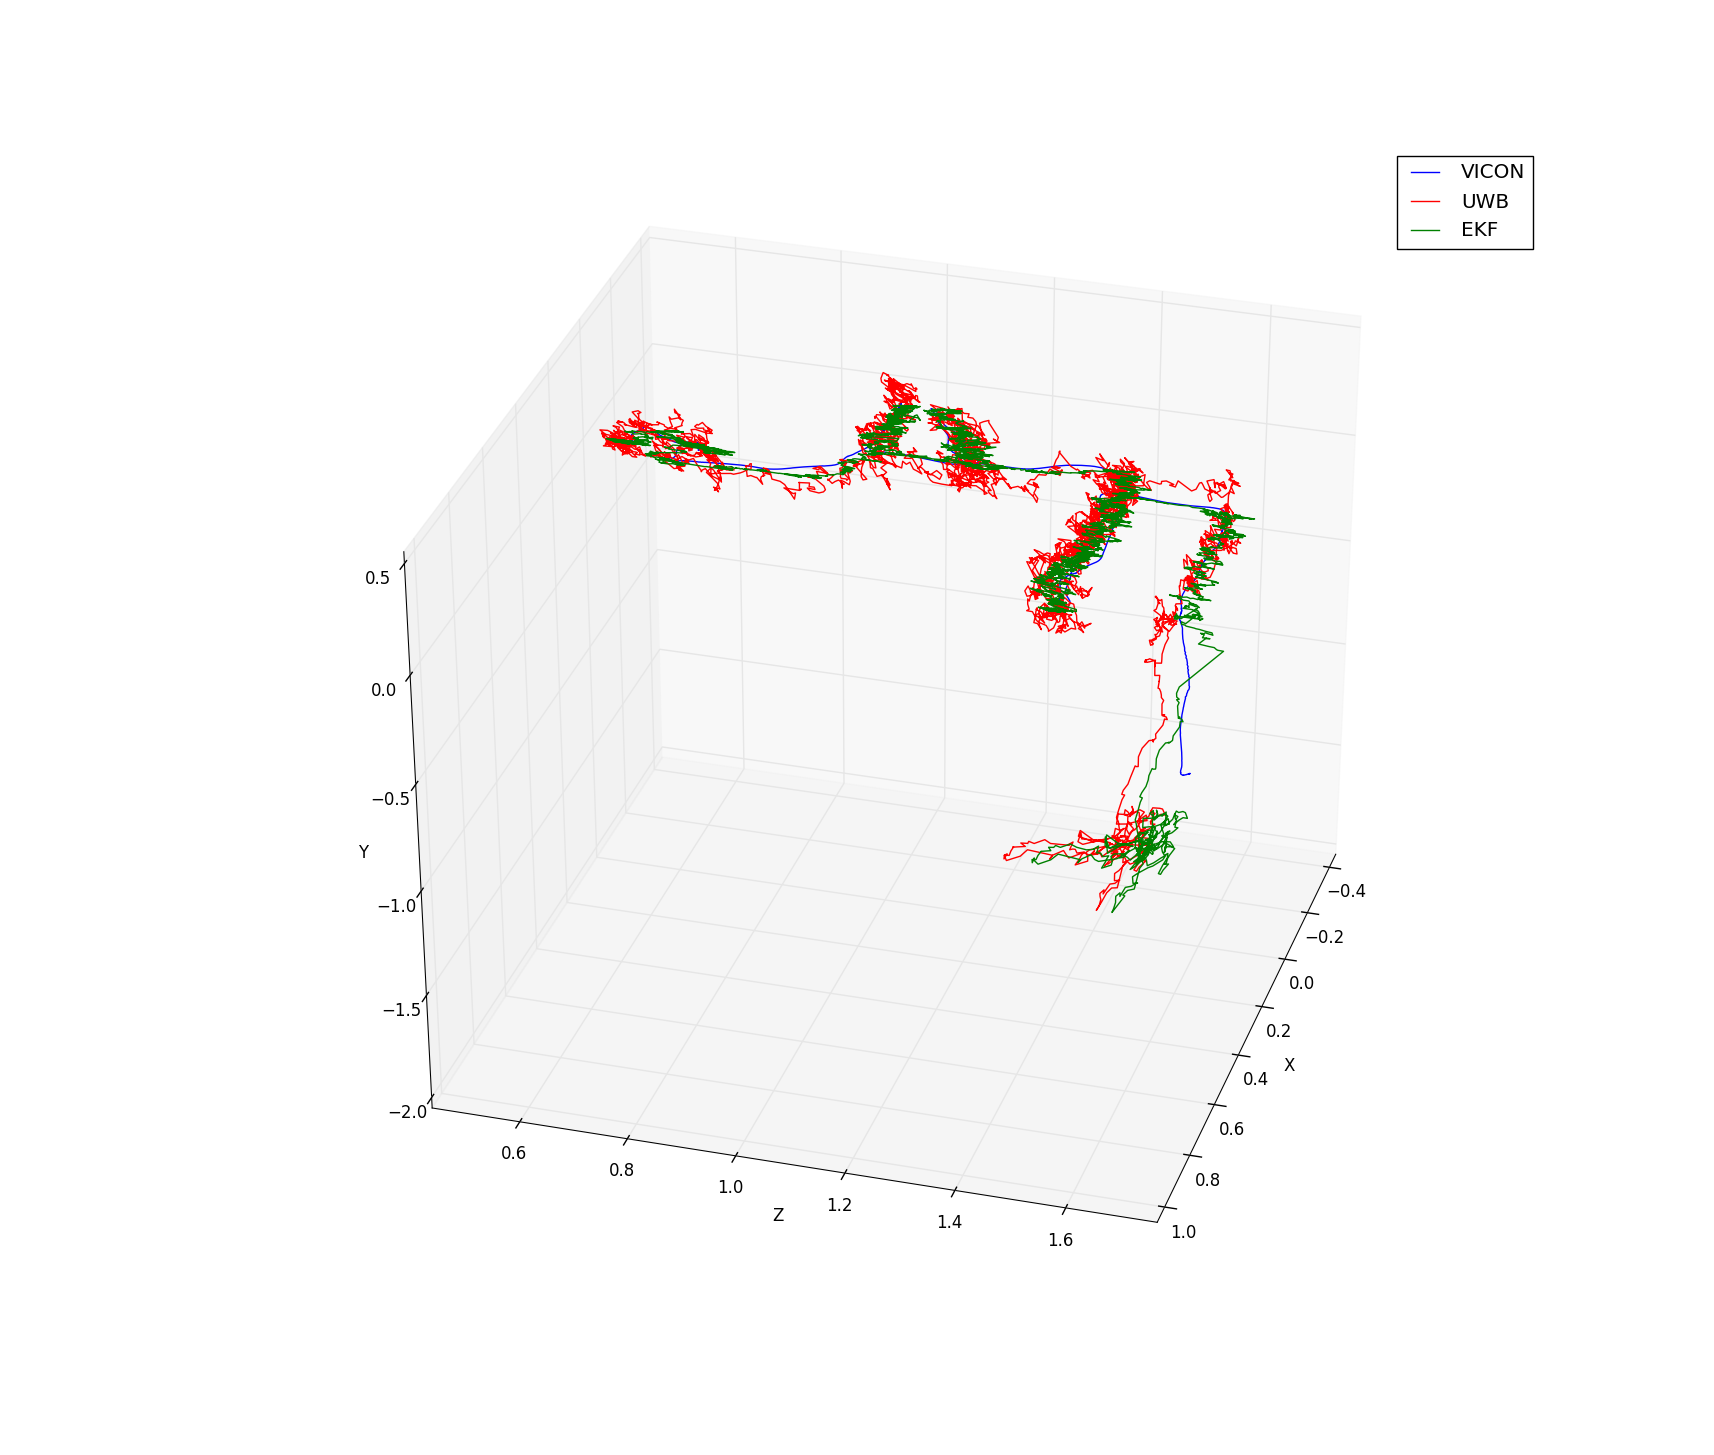
\includegraphics[width=1.0\textwidth]{figures/evaluation}
	\caption{3D plot of the coordinate points measured by the \ac{UWB} system (red), the points measured by the VICON system (magenta) and the fused positions (green) of the experiment number 1.}\label{fig:evaluation}
\end{figure}

\begin{figure}[ht!]\centering
	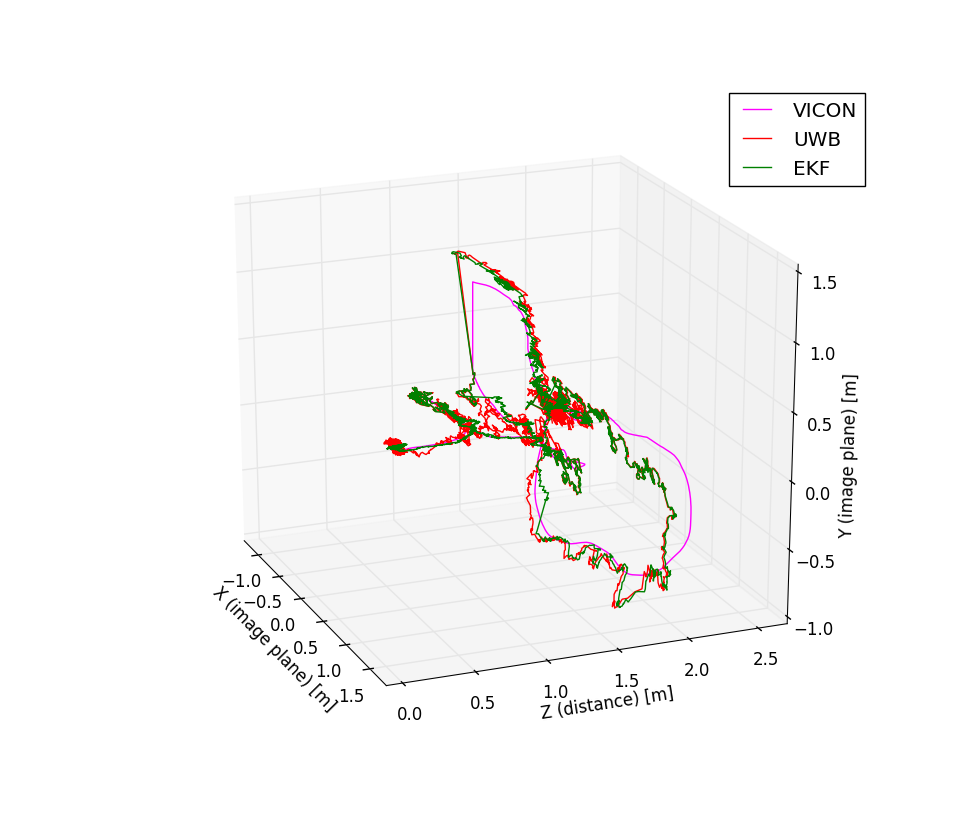
\includegraphics[width=1.0\textwidth]{figures/evaluation_redetect}
	\caption{3D plot of the coordinate points measured by the \ac{UWB} system (red), the points measured by the VICON system (magenta) and the fused positions (green) of the experiment number 5 in which the object goes several times out of the camera view and the visual tracker has to re-detect the object.}\label{fig:evaluation_redetect}
\end{figure}
